\chapter{Analyse}

Als Grundlage für die RadioTour Applikation dient aus Sicht der Funktionalität die bestehende Web Applikation. Daraus werden die Requirements und UseCases erzeugt. Im folgenden werden die einzelnen Teile der Analyse vorgestellt.

\section{Struktur der Applikation}
%ja, plural ist Status, http://de.wikipedia.org/wiki/Status
Die Applikation hat im Grunde zwei Status, einerseits werden vor dem Rennen die Fahrerliste und die Marschtabelle importiert andererseits wird die Rennsituation während dem Rennen erfasst und Änderungen festgehalten. Diese beiden Status können aber nicht absolut voneinander getrennt werden, da während dem Rennen Änderungen denkbar sind. So entsteht die Baumartige Struktur, wie sie in der Abbildung zu sehen ist.

\begin{figure}[h!]
\caption{Struktur der Applikation}
\centering
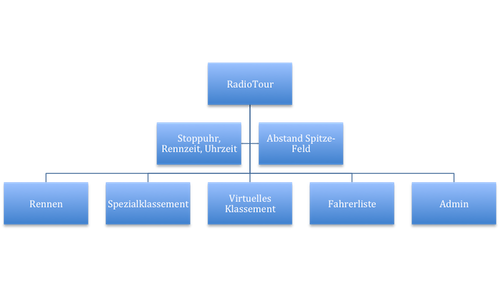
\includegraphics{05technischerbericht/images/struktur.png}
\end{figure} 


\section{Technologien}
\subsection{Android}
Die native Programmiersprache für das Android Betriebssystem ist Java. Die Programmierung in Java bringt den Vorteil, dass auf die gesamte \gls{api} von Android zugegriffen werden kann. Weiter sind die Geräte genau dafür ausgelegt und die optimale Performance kann erreicht werden. Sämtliche Komponenten dieser Arbeit sind in Java geschrieben. Für die Persistierung der Daten auf dem Tablet wird eine \gls{sqlite} Datenbank verwendet.

\subsection{Externe Libraries}
Android beinhaltet bereits ein umfangreiches Framework zur Entwicklung. Einzig beim \gls{orm}, also beim Abbilden von Objektdaten in der Datenbank kommt eine externe Library zum Einsatz.
\\
\textit{ORMLite} \footnote{ORMLite, \url{http://ormlite.com/}, Aufgerufen am 23.05.2012} ist eine OpenSource Java Library, welche auch für Android eine optimale Lösung bietet. Die zu verwendenden Felder einer Klasse können mit Java Annotationen versehen werden, daraus versucht ORMLite dann die Datenbank zu beschreiben. In der RadioTour Anwendung konnten alle Felder abgebildet werden.


\subsection{Entwicklungsumgebung}
Die von Android empfohlene Entwicklungsumgebung ist Eclipse\footnote{Eclipse, \url{http://eclipse.org/}} mit einem Plugin zur Entwicklung von Android Applikationen. Auf der Entwicklerseite von Android steht dazu folgendes:
\begin{quote}
\grqq Android Development Tools (ADT) is a plugin for the Eclipse IDE that is designed to give you a powerful, integrated environment in which to build Android applications.\grqq
\footnote{Android Plugin für Eclipse, \url{http://developer.android.com/sdk/eclipse-adt.html}}
\end{quote}
Eclipse ist eine weit verbreitete \gls{ide} und wird aktiv weiter entwickelt. Mit dem Plugin zusammen bilden Sie eine solide Grundlage für dieses Projekt.
\\
Damit die Android Applikation direkt auf dem Computer getestet werden kann, stellt Google ein Emulator zur Verfügung. Der Emulator ist allerdings auch als solcher zu betrachten da die Bedienung nicht vergleichbar ist mit einem richtigen Tablet.

\subsection{Android Version}
Eine Anwendung wird für eine spezifische Android Version entwickelt und getestet, somit kann garantiert werden, dass das Verhalten der Anwendung  immer gleich ist. In dieser Arbeit ist dies die Version 3.1 mit dem Versionsnamen \textit{Honeycomb}.\footnote{\url{Android Version Honeycomb, http://de.wikipedia.org/wiki/Android_(Betriebssystem)\#Versionsverlauf}}.
\\
Die Entwicklung auf einer Version schliesst jedoch nicht aus, dass die Anwendung in neueren Versionen nicht mehr lauffähig ist. Auch \textit{RadioTour} kann für zukünftige Versionen weiterentwickelt und verwendet werden.

\section{Mitbewerberanalyse}
Die Art der Applikation ist sehr spezifisch und kann nicht direkt auf andere Sportereignisse angewendet werden. Deshalb beinhaltet die Analyse von Mitbewerbern nur die grossen europäischen Radrennen. Wie bei der Tour de Suisse ist auch in Frankreich an der \textit{Tour de France}\footnote{Tour de France, \url{http://www.letour.fr/}} ein RadioTour Speaker mit dabei. Darüber wie die Aufzeichnungen in Frankreich im genauen stattfinden kann aber nur spekuliert werden da die Informationen nicht öffentlich zugänglich sind.
\\
In Italien findet zum Zeitpunkt dieser Arbeit der \textit{Giro d'Italia}\footnote{Giro d'Italia, \url{http://www.gazzetta.it/Speciali/Giroditalia/2012/}} statt. Bei diesem Radrennen ist es möglich aus den Informationen, welche auf der Webseite verfügbar sind, zu schliessen, dass ein ähnliches System verwendet wird. Während dem Rennen ist es möglich die aktuelle Rennsituation zu betrachten.

\begin{figure}[h!]
\caption{Rennsituation am Giro d'Italia}
\label{fig:giro}
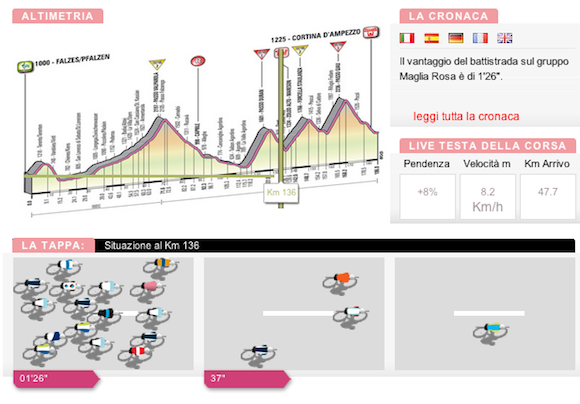
\includegraphics[scale=0.7]{05technischerbericht/images/giro.png}
\end{figure} 

In der Abbildung \ref{fig:giro} ist der Live Abschnitt der offiziellen Webseite zu sehen. Im oberen Teil wird der Standort in der aktuelle Etappe eingeblendet. Weiter unten ist die Situation an der Spitze abgebildet. Die Fahrer sind nach Rückstand gruppiert.
\\
Da jedoch nicht zu erkennen ist, wie die Informationen im Feld erfasst werden muss die Mitbewerberanalyse an dieser Stelle abgeschlossen werden.

\chapter{Architektur}
Im folgenden Abschnitt wird die Architektur der Applikation diskutiert. Die Architektur ist so gewählt, dass die einzelnen funktionalen Komponenten zueinander eine tiefe Abhängigkeit aufweisen.

\section{Domainmodel}
Die Domainlogik beinhaltet die Kernelemente der Applikation. Einerseits sind dies die Rennfahrer, welche Informationen über sich festhalten andererseits die Etappe mit den Informationen zur Strecke. Während dem Rennen werden die Fahrer in Gruppen unterteilt. Auch diese Gruppen sind in der Domain abgebildet. Das Klassendiagramm des Domain Package zeigt die wesentlichen Elemente.

\begin{figure}[h!]
\caption{Die Domainklassen in der Abhängigkeit}
\label{fig:domain}
\centering
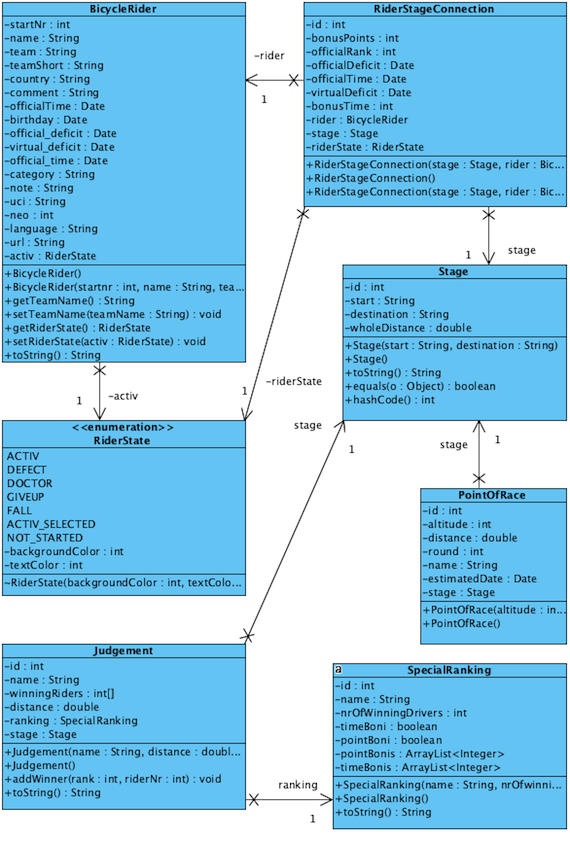
\includegraphics{05technischerbericht/images/domain.png}
\end{figure} 


\textit{BicycleRider} speichert die Angaben zu einem Fahrer und beinhaltet keine eigene Logik. Ein Fahrer hat immer genau ein \textit{RiderState}. Dies ist ein Java \gls{enum} und zeigt den Status des Fahrer an. Nach dem Import der Fahrerliste werden alle Fahrer auf \textit{activ} gesetzt.

In \textit{Stage} ist die Etappe definiert. Jede Etappe hat eine Marschtabelle in Form von mehreren \textit{PointOfRace} Objekten. Diese Objekte werden durch Import der Marschtabelle erstellt.
Da pro Etappe jeder \textit{BicycleRider} einen anderen \textit{RiderState} haben kann, gibt es die Verbindungsklasse \textit{RiderStageConnection}. In dieser Klasse ist jeweils die Etappe mit dem Fahrer verknüpft. Dies ermöglicht es den Rückstand eines Fahrers in mehreren Etappen zu verfolgen.
Ein \textit{Judgement}, also eine Wertung, gehört immer zu einer Etappe. Diese Wertungen sind definiert durch ein \textit{SpecialRanking}, welche Punkte- und Zeitboni beinhalten können.


\chapter{Realisierung}
Lorem ipsum dolor sit amet, consetetur sadipscing elitr, sed diam nonumy eirmod tempor invidunt ut labore et dolore magna aliquyam erat, sed diam voluptua. At vero eos et accusam et justo duo dolores et ea rebum. Stet clita kasd gubergren, no sea takimata sanctus est Lorem ipsum dolor sit amet. Lorem ipsum dolor sit amet, consetetur sadipscing elitr, sed diam nonumy eirmod tempor invidunt ut labore et dolore magna aliquyam erat, sed diam voluptua. At vero eos et accusam et justo duo dolores et ea rebum. Stet clita kasd gubergren, no sea takimata sanctus est Lorem ipsum dolor sit amet.

\chapter{Testing}
Lorem ipsum dolor sit amet, consetetur sadipscing elitr, sed diam nonumy eirmod tempor invidunt ut labore et dolore magna aliquyam erat, sed diam voluptua. At vero eos et accusam et justo duo dolores et ea rebum. Stet clita kasd gubergren, no sea takimata sanctus est Lorem ipsum dolor sit amet. Lorem ipsum dolor sit amet, consetetur sadipscing elitr, sed diam nonumy eirmod tempor invidunt ut labore et dolore magna aliquyam erat, sed diam voluptua. At vero eos et accusam et justo duo dolores et ea rebum. Stet clita kasd gubergren, no sea takimata sanctus est Lorem ipsum dolor sit amet.

\chapter{Ergebnisse und Schlussfolgerungen}
Lorem ipsum dolor sit amet, consetetur sadipscing elitr, sed diam nonumy eirmod tempor invidunt ut labore et dolore magna aliquyam erat, sed diam voluptua. At vero eos et accusam et justo duo dolores et ea rebum. Stet clita kasd gubergren, no sea takimata sanctus est Lorem ipsum dolor sit amet. Lorem ipsum dolor sit amet, consetetur sadipscing elitr, sed diam nonumy eirmod tempor invidunt ut labore et dolore magna aliquyam erat, sed diam voluptua. At vero eos et accusam et justo duo dolores et ea rebum. Stet clita kasd gubergren, no sea takimata sanctus est Lorem ipsum dolor sit amet.